% MORPH — MHCTransformerBlock Detail (Diagram 2)
% Shows the 3-channel mHC residual stream through one block.
% Compile: pdflatex morph_block.tex

\documentclass[border=14pt]{standalone}
\usepackage[T1]{fontenc}
\usepackage{tikz}
\usetikzlibrary{
  arrows.meta, fit, positioning, calc,
  backgrounds, decorations.pathreplacing,
}

% ── Palette ──────────────────────────────────────────────────────────────────
\definecolor{cbBlue}{HTML}{4477AA}
\definecolor{cbOrange}{HTML}{EE7733}
\definecolor{cbPurple}{HTML}{AA3377}

\definecolor{fBlue}{HTML}{DCEAF7}
\definecolor{fOrange}{HTML}{FDE8D0}
\definecolor{fPurple}{HTML}{EEDCEE}
\definecolor{fGray}{HTML}{EBEBEB}

\definecolor{chComp}{HTML}{7BAFD4}   % compute channel stripe
\definecolor{chCtx}{HTML}{F4B183}    % context channel stripe
\definecolor{chMem}{HTML}{C9A0C9}    % memory channel stripe

\definecolor{bdr}{HTML}{555555}

% ── Styles ───────────────────────────────────────────────────────────────────
\tikzset{
  B/.style={draw=bdr, thick, rounded corners=4pt,
    minimum width=6.0cm, minimum height=1.0cm,
    font=\small\sffamily, align=center, inner sep=5pt},
  Bs/.style={B, minimum height=0.6cm, font=\footnotesize\sffamily},
  A/.style={-{Stealth[length=2.5mm,width=2mm]}, thick},
  Ad/.style={-{Stealth[length=2.2mm,width=1.8mm]}, thick, densely dashed},
  Ar/.style={-{Stealth[length=2.5mm,width=2mm]}, thick, rounded corners=5pt},
  ph/.style={font=\small\sffamily\bfseries},
  sub/.style={font=\scriptsize\sffamily},
  tiny/.style={font=\tiny\sffamily},
}

% Channel stripe: a 3-part colored bar
\newcommand{\channelbar}[2]{%
  % #1 = center coordinate name, #2 = total width
  \fill[chComp] ([xshift=-#2/2]#1) rectangle ([xshift=-#2/2+#2*0.5]#1 |- {([yshift=0.25cm]#1)});
  \fill[chCtx]  ([xshift=-#2/2+#2*0.5]#1) rectangle ([xshift=-#2/2+#2*0.833]#1 |- {([yshift=0.25cm]#1)});
  \fill[chMem]  ([xshift=-#2/2+#2*0.833]#1) rectangle ([xshift=#2/2]#1 |- {([yshift=0.25cm]#1)});
}

\begin{document}
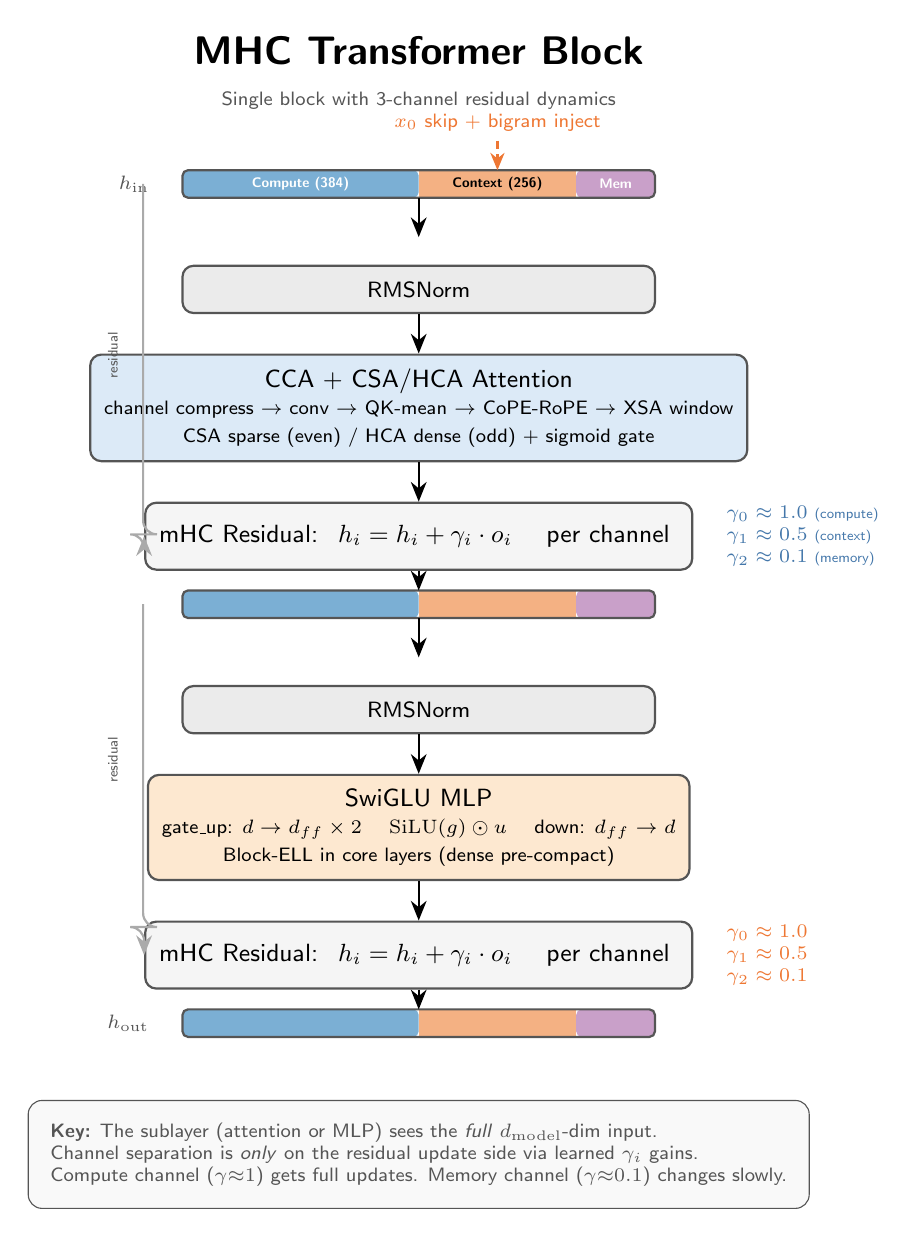
\begin{tikzpicture}[node distance=0.55cm]

% ── Title ────────────────────────────────────────────────────────────
\node[font=\Large\sffamily\bfseries] (title) {MHC Transformer Block};
\node[sub, text=bdr, below=0.1cm of title] (subtitle)
  {Single block with 3-channel residual dynamics};

% =====================================================================
% RESIDUAL STREAM: 3-channel colored bars
% =====================================================================

% Input stream bar
\coordinate (stream_in) at ($(subtitle.south)+(0,-1.0)$);

% Draw channel bars as rectangles
\newcommand{\barW}{6.0cm}
\newcommand{\barH}{0.35cm}
\newcommand{\compF}{0.5}    % 384/768
\newcommand{\ctxF}{0.333}   % 256/768
\newcommand{\memF}{0.167}   % 128/768

% ── Input bar ────────────────────────────────────────────────────────
\coordinate (bar_in_left) at ($(stream_in)+(-3.0,0)$);
\fill[chComp, rounded corners=2pt]
  (bar_in_left) rectangle ++(3.0, \barH);
\fill[chCtx]
  ($(bar_in_left)+(3.0, 0)$) rectangle ++(2.0, \barH);
\fill[chMem, rounded corners=2pt]
  ($(bar_in_left)+(5.0, 0)$) rectangle ++(1.0, \barH);
\draw[bdr, thick, rounded corners=2pt]
  (bar_in_left) rectangle ++(6.0, \barH);

% Labels on input bar
\node[font=\tiny\sffamily\bfseries, text=white] at ($(bar_in_left)+(1.5,0.175)$)
  {Compute (384)};
\node[font=\tiny\sffamily\bfseries] at ($(bar_in_left)+(4.0,0.175)$)
  {Context (256)};
\node[font=\tiny\sffamily\bfseries, text=white] at ($(bar_in_left)+(5.5,0.175)$)
  {Mem};

\node[sub, text=bdr, anchor=east] at ($(bar_in_left)+(-0.3,0.175)$) {$h_{\mathrm{in}}$};

% Arrow down from bar to RMSNorm
\coordinate (bar_in_mid) at ($(bar_in_left)+(3.0, 0)$);
\draw[A] (bar_in_mid) -- ++(0,-0.5);

% ── RMSNorm (Attention) ─────────────────────────────────────────────
\node[Bs, fill=fGray, below=0.85cm of stream_in] (norm_a) {RMSNorm};

% ── CCA Attention ────────────────────────────────────────────────────
\node[B, fill=fBlue, below=0.5cm of norm_a, minimum height=1.3cm] (attn) {
  CCA + CSA/HCA Attention\\[-1pt]
  {\scriptsize channel compress $\to$ conv $\to$ QK-mean $\to$
  CoPE-RoPE $\to$ XSA window}\\[-1pt]
  {\scriptsize CSA sparse (even) / HCA dense (odd) + sigmoid gate}
};
\draw[A] (norm_a) -- (attn);

% ── mHC Residual (Attention) ────────────────────────────────────────
\node[B, fill=fGray!50, below=0.5cm of attn, minimum height=0.85cm] (mhc_a) {
  mHC Residual: \ $h_i = h_i + \gamma_i \cdot o_i$ \quad per channel
};
\draw[A] (attn) -- (mhc_a);

% Gamma annotations for attention residual
\node[sub, text=cbBlue, right=0.3cm of mhc_a, align=left, anchor=west]
  (ga_lbl) {$\gamma_0 \approx 1.0$ {\tiny(compute)}\\
  $\gamma_1 \approx 0.5$ {\tiny(context)}\\
  $\gamma_2 \approx 0.1$ {\tiny(memory)}};

% Skip connection: bar_in → mhc_a (residual)
\draw[A, bdr!50, rounded corners=5pt]
  ($(bar_in_left)+(-0.5, 0.175)$) -- ++(0, -4.45) -| (mhc_a.west);
\node[tiny, text=bdr, rotate=90, anchor=south] at ($(bar_in_left)+(-0.7,-2.0)$) {residual};

% ── Mid stream bar ──────────────────────────────────────────────────
\coordinate (stream_mid) at ($(mhc_a.south)+(0,-0.6)$);
\coordinate (bar_mid_left) at ($(stream_mid)+(-3.0,0)$);
\fill[chComp, rounded corners=2pt]
  (bar_mid_left) rectangle ++(3.0, \barH);
\fill[chCtx]
  ($(bar_mid_left)+(3.0, 0)$) rectangle ++(2.0, \barH);
\fill[chMem, rounded corners=2pt]
  ($(bar_mid_left)+(5.0, 0)$) rectangle ++(1.0, \barH);
\draw[bdr, thick, rounded corners=2pt]
  (bar_mid_left) rectangle ++(6.0, \barH);

\draw[A] (mhc_a.south) -- ++(0,-0.25);

% ── RMSNorm (MLP) ───────────────────────────────────────────────────
\coordinate (bar_mid_bot) at ($(bar_mid_left)+(3.0, 0)$);
\draw[A] (bar_mid_bot) -- ++(0,-0.5);

\node[Bs, fill=fGray, below=0.85cm of stream_mid] (norm_m) {RMSNorm};

% ── SwiGLU MLP ──────────────────────────────────────────────────────
\node[B, fill=fOrange, below=0.5cm of norm_m, minimum height=1.1cm] (mlp) {
  SwiGLU MLP\\[-1pt]
  {\scriptsize gate\_up: $d \to d_{ff} \times 2$ \quad
  $\mathrm{SiLU}(g) \odot u$ \quad down: $d_{ff} \to d$}\\[-1pt]
  {\scriptsize Block-ELL in core layers (dense pre-compact)}
};
\draw[A] (norm_m) -- (mlp);

% ── mHC Residual (MLP) ──────────────────────────────────────────────
\node[B, fill=fGray!50, below=0.5cm of mlp, minimum height=0.85cm] (mhc_m) {
  mHC Residual: \ $h_i = h_i + \gamma_i \cdot o_i$ \quad per channel
};
\draw[A] (mlp) -- (mhc_m);

% Gamma annotations for MLP residual
\node[sub, text=cbOrange, right=0.3cm of mhc_m, align=left, anchor=west]
  {$\gamma_0 \approx 1.0$\\$\gamma_1 \approx 0.5$\\$\gamma_2 \approx 0.1$};

% Skip connection: mid_bar → mhc_m (residual)
\draw[A, bdr!50, rounded corners=5pt]
  ($(bar_mid_left)+(-0.5, 0.175)$) -- ++(0, -4.1) -| (mhc_m.west);
\node[tiny, text=bdr, rotate=90, anchor=south] at ($(bar_mid_left)+(-0.7,-1.8)$) {residual};

% ── Output stream bar ───────────────────────────────────────────────
\coordinate (stream_out) at ($(mhc_m.south)+(0,-0.6)$);
\coordinate (bar_out_left) at ($(stream_out)+(-3.0,0)$);
\fill[chComp, rounded corners=2pt]
  (bar_out_left) rectangle ++(3.0, \barH);
\fill[chCtx]
  ($(bar_out_left)+(3.0, 0)$) rectangle ++(2.0, \barH);
\fill[chMem, rounded corners=2pt]
  ($(bar_out_left)+(5.0, 0)$) rectangle ++(1.0, \barH);
\draw[bdr, thick, rounded corners=2pt]
  (bar_out_left) rectangle ++(6.0, \barH);

\draw[A] (mhc_m.south) -- ++(0,-0.25);

\node[sub, text=bdr, anchor=east] at ($(bar_out_left)+(-0.3,0.175)$) {$h_{\mathrm{out}}$};

% =====================================================================
% SIDE INJECTIONS (into context channel)
% =====================================================================

% x₀ skip → context channel of input bar
\coordinate (ctx_in) at ($(bar_in_left)+(4.0, 0.175)$);
\node[sub, text=cbOrange, anchor=south, align=center]
  at ($(ctx_in)+(0, 0.55)$) (x0_lbl) {$x_0$ skip + bigram inject};
\draw[Ad, cbOrange] (x0_lbl.south) -- ($(ctx_in)+(0,0.175)$);

% =====================================================================
% KEY INSIGHT BOX
% =====================================================================

\node[draw=bdr, rounded corners=5pt, fill=fGray!30,
      minimum width=6.5cm, inner sep=8pt, align=left,
      font=\scriptsize\sffamily, text=bdr,
      below=0.8cm of stream_out] (insight) {
  \textbf{Key:} The sublayer (attention or MLP) sees the \emph{full}
  $d_{\mathrm{model}}$-dim input.\\
  Channel separation is \emph{only} on the residual update side via
  learned $\gamma_i$ gains.\\
  Compute channel ($\gamma{\approx}1$) gets full updates.
  Memory channel ($\gamma{\approx}0.1$) changes slowly.
};

\end{tikzpicture}
\end{document}
